\chapter{Case~Study: An~IDE~for~Research}

While the first case study focused on a system with several complex, deadline-driven workflows, it had only a simple notion of roles. The second case study balances this by focusing on an application that has a simple and well-known workflow, but a more complex notion of user roles.

\sectionnote {AC}
\section {Background}
\label{sec:case-study-research-background}

Taverna is an open source workflow management tool which aids in the execution of scientific experiments with a focus on in silico experiments. In silico experiments are scientific experiments which are done entirely on a computer such as complex models of cells. The main benefit to in silico experiments is the increased precesion and the size of the data that can be generated and analyzed. Unfortunately, many researchers are not programmers and are unable to easily create in silico experimentats. Taverna allows a researcher to describe an experiment with a workflow so that the steps of an experiment are abstracted from the programming of it. This modular workflow approach allows a researcher to design an experiment without having to worry about the technical details of programming.

Due to the large computational requirement of in silico experiments Taverna allows multiple systems to work on the computations of a single experiment. This allows a researcher to utilize an entire network of computers and benefit from the extra computational power. Because of the nature many scientific experiments many tasks are able to be done in parallel. With parallel activities and enough computational power the speed at which an experiment can be completed drastically increases.

Another workflow tool we found in the scientific domain is Pegasus, which is similar to Taverna and provides all the same features. However, Taverna and Pegasus do not offer any tools to write proper scientific documentation following the scientific method. Our second case study differs from these tools in that we handle the act of documenting scientific experiments and not the act of executing the experiment itself.

\sectionnote {BM}
\section {Overview}
\label{sec:case-study-research-overview}

Scientific misconduct and issues with reproducibility are a growing concern.
While deliberate misconduct and fraud are difficult to prevent using technological means, it should be possible to encourage adequate record-keeping and proper process by using a software tool to guide inexperience researchers through the scientific process.

In general, the process of performing a research project can be described in six steps:
\begin{compactenum}
\item \textbf{Write a hypothesis}
\item \textbf{Perform a literature review} to discover prior work in the field, summarize the context of the work, and perhaps gain ideas for design of the experiment.
\item \textbf{Design an experimental method} to test the hypothesis.
\item \textbf{Record the results} obtained from the experiment.
\item \textbf{Analyze the results}, often using a set of domain-specific tools.
\item \textbf{Draw conclusions} from the analysis.
\end{compactenum}

Though the process is often taught as a sequence of steps, some iteration may occur occasionally; for example, while designing the method a researcher might realize that their hypothesis as written is unclear or difficult, and alter it to correct the issue. On the other hand, there are several patterns of changes that should not be made, in order to avoid introducing biases or outright fraud:
\begin{compactitem}
\item the hypothesis and method should not be edited after the experiment begins;
\item the results should not be changed after beginning analysis;
\item the analysis, conclusions, and literature review should always be editable.
\end{compactitem}

The research process itself may be carried out by a number of individuals with different responsibilities, depending on the discipline. For example, a technician may be responsible for validating the methodology and carrying out the experiment itself, while a statistician may be consulted for the analysis. It is important that a tool for managing the research process can accommodate any arbitrary assignment of responsibilities to individuals that a project demands.

As a well-defined sequence of steps with restricted iteration, this process seems like an excellent candidate for automation using a workflow framework. Furthermore, as user roles are not predefined, but instead specified on a project-by-project basis, this case study provides an opportunity to investigate best practices and existing libraries for role-based access.



\sectionnote {AC}
\section {Requirements}

  Figures \ref{fig:case-research-use-case-project-management} through \ref{fig:case-research-use-case-project-workflow} display the individual use cases for the research IDE application. They have been separated into two diagrams based on project management and the main project workflow. The project management shown in Figure \ref{fig:case-research-use-case-project-management} goes over which actors have permission to view, create and delete research projects. In addition, it also displays modifying the permissions of users for a given project and how the project advances to the next stage of the workflow. The project workflow shown in Figure \ref{fig:case-research-use-case-project-workflow} focuses on the workflow system described in section \ref{sec:case-study-research-overview}.

\begin{figure}[!ht]
\centering 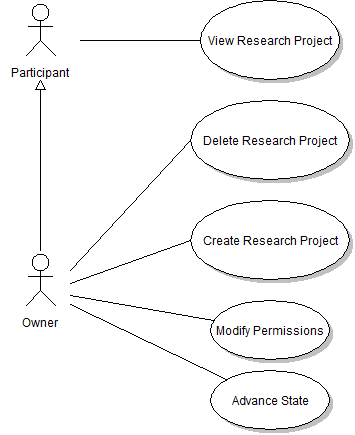
\includegraphics[height=5in]{./img/case-study-research-railgun/project_management_use_case}
\caption{Use case diagram for the project management functionality of the research IDE.}
\label{fig:case-research-use-case-project-management}
\end{figure}

\begin{figure}[!ht]
\centering 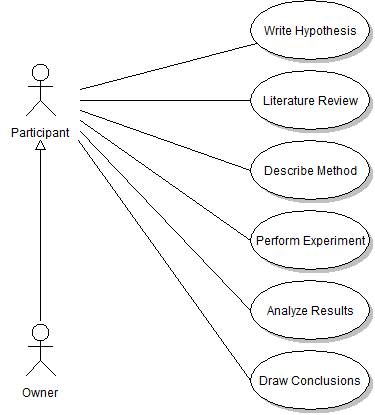
\includegraphics[height=5in]{./img/case-study-research-railgun/project_workflow_use_case}
\caption{Use case diagram for the project workflow functionality of the research IDE.}
\label{fig:case-research-use-case-project-workflow}
\end{figure}

\FloatBarrier

  The two actors Owner and Participant represent the two roles in the research IDE. Owners own projects and participants participate in projects. Any user is able to create a project which then assigns their role as the owner of that project. As an owner of a project the user has all permissions granted to them and is able to grant permissions to participants for specific stages of the workflow. There are two permission types: view, and edit. The view permission allows access to view specific stages of a workflow and the edit permission allows a participant to make modifications to the project in that stage of the workflow.

  Tables \ref{tbl:use-case-view-research-project} to \ref{tbl:use-case-advance-state} display the use case descriptions for the project management diagram shown above. Tables \ref{tbl:use-case-write-hypothesis} to \ref{tbl:use-case-draw-conclusions} display the use case descriptions for the above project workflow diagram. These descriptions describe exactly what permissions are required to do actions during each use case.
 
\begin{table}
  \centering
  \caption{Use case description for the ``View Research Project'' use case of the research IDE system.}
  \label{tbl:use-case-view-research-project}

  \begin{usecase}[View Research Project]
    \ucpart{Description}
    A User can view information about a project that he has permissions with.
    %
    \ucpart{Actors}
    Owner, Participant
    %
    \ucpart{Preconditions}
    The Research Project Exists and the User accessing it has at least one permission to view a task in the project.
    %
    \ucpart{Flow}
    \ucnormal
    \begin{ucenum}
      \item The User selects a research project from a list of projects that the User has access to.
      \item The User is shown detailed information about the project: current state of project, and any sections the user is allowed to view/edit.
    \end{ucenum}
    %
    \ucpart{Exceptions}
    \ucexception{No Permissions}
    The User has no permissions to view the project and is redirected back to a list of projects he has permission to view and an error is shown.
    %
    \ucpart{Postconditions}
    The User is brought to a details view of the selected project.
  \end{usecase}
\end{table}


\begin{table}
  \centering
  \caption{Use case description for the ``Delete Research Project'' use case of the research IDE system.}
  \label{tbl:use-case-delete-research-project}

  \begin{usecase}[Delete Research Project]
    \ucpart{Description}
    A Research Project can be deleted by the Owner of that project at any time.
    %
    \ucpart{Actors}
    Owner
    %
    \ucpart{Preconditions}
    The Research Project to be deleted exists.
    %
    \ucpart{Flow}
    \ucnormal
    \begin{ucenum}
      \item The User selects to delete the project.
      \item A confirmation box appears and the User agrees.
      \item The Project is deleted and the User is sent to a list of projects he has permission to view.
    \end{ucenum}
    %
    \ucpart{Variations}
    \ucbranch{A}
    \begin{ucenum}
      \item [A.2] A confirmation box appears and the User disagrees.
      \item [A.3] The User returns the the details view of that project.
    \end{ucenum}
    %
    \ucpart{Exceptions}
    \ucexception{Not Owner}
    A participant cannot delete a project he does not own. He is redirected back to the list of projects he has permission to view.
    %
    \ucpart{Postconditions}
    The Research Project is deleted from the system.
  \end{usecase}
\end{table}


\begin{table}
  \centering
  \caption{Use case description for the ``Create Research Project'' use case of the research IDE system.}
  \label{tbl:use-case-create-research-project}

  \begin{usecase}[Create Research Project]
    \ucpart{Description}
    A Research Project can be created by any User and that User becomes the Owner of that project.
    %
    \ucpart{Actors}
    Owner
    %
    \ucpart{Flow}
    \ucnormal
    \begin{ucenum}
      \item The User selects to Create a new Research Project.
      \item The User submits a name and description for the project.
      \item The Research project is created, The User is assigned as the owner and is redirected to viewing the project.
    \end{ucenum}
    %
    \ucpart{Postconditions}
    The Research Project is created and the User is assigned to the Owner of the project.
  \end{usecase}
\end{table}


\begin{table}
  \centering
  \caption{Use case description for the ``Modify Permissions'' use case of the research IDE system.}
  \label{tbl:use-case-modify-permissions}

  \begin{usecase}[Modify Permissions]
    \ucpart{Description}
    The Owner of a project can modify the permissions of other Users for his project.
    %
    \ucpart{Actors}
    Owner
    %
    \ucpart{Preconditions}
    The User is the Owner of the project to which he is assigned permissions.
    %
    \ucpart{Flow}
    \ucnormal
    \begin{ucenum}
      \item The User selects to modify the permissions for his project.
      \item A list of other Users on the system is shown along with their current.
      \item The User selects a specific permission to modify and submits the change.
      \item The other User now has the selected permissions for the project.
    \end{ucenum}
    %
    \ucpart{Exceptions}
    \ucexception{Cannot Modify Owner Permissions}
    The Owner always has every permission and this cannot be changed, redirected back to project view.
    \ucexception{Not Owner}
    Only Owners can modify permissions, redirected back to project view.
    %
    \ucpart{Postconditions}
    The User who had his permissions modified can now do any actions that require that permission.
  \end{usecase}
\end{table}


\begin{table}
  \centering
  \caption{Use case description for the ``Advance State'' use case of the research IDE system.}
  \label{tbl:use-case-advance-state}

  \begin{usecase}[Advance State]
    \ucpart{Description}
    The Owner can advance the state of the project as long as something has been saved into the current state.
    %
    \ucpart{Actors}
    Owner
    %
    \ucpart{Preconditions}
    There is another state in the workflow after the current state.
    %
    \ucpart{Flow}
    \ucnormal
    \begin{ucenum}
      \item The User selects to advance the state of the project
      \item There is something saved for the current state and the state is advanced to the next state in the workflow.
    \end{ucenum}
    %
    \ucpart{Variations}
    \ucbranch{A}
    \begin{ucenum}
      \item [A.2] There is nothing saved for the current state and a message is shown notifying the User that something must be saved before moving on.
    \end{ucenum}
    %
    \ucpart{Exceptions}
    \ucexception{Not Owner}
    A participant cannot advance the state of a project. He is redirected back to the project view
    \ucexception{Last State}
    There is no state after the current state so the state cannot be advanced, User is redirected back to project view.
    %
    \ucpart{Postconditions}
    The state of the workflow is advanced to the next state.
  \end{usecase}
\end{table}


\begin{table}
  \centering
  \caption{Use case description for the ``Write Hypothesis'' use case of the research IDE system.}
  \label{tbl:use-case-write-hypothesis}

  \begin{usecase}[Write Hypothesis]
    \ucpart{Description}
    A User with the correct permissions can edit or view the hypothesis of the current project.
    %
    \ucpart{Actors}
    Owner, Participant
    %
    \ucpart{Preconditions}
    The workflow must be in the ‘Write Hypothesis”, “Literature Review” or “Describe Method” state. The User has the ‘edit’ or ‘view’ permission for this task.
    %
    \ucpart{Flow}
    \ucnormal
    \begin{ucenum}
      \item The User selects to write the hypothesis.
      \item The User has the ‘edit’ permission and makes a modification to the hypothesis and selects to save.
      \item The Hypothesis is updated and saved.
    \end{ucenum}
    %
    \ucpart{Variations}
    \ucbranch{A}
    \begin{ucenum}
      \item [A.2] The User has the ‘view’ permission and does not have the ‘edit’ permission and is shown the current hypothesis.
    \end{ucenum}
    %
    \ucpart{Exceptions}
    \ucexception{No Permission}
    The User does not have permission to ‘edit’ or ‘view’ the hypothesis and is returned to project view.
  \end{usecase}
\end{table}


\begin{table}
  \centering
  \caption{Use case description for the ``Literature Review'' use case of the research IDE system.}
  \label{tbl:use-case-literature-review}

  \begin{usecase}[Literature Review]
    \ucpart{Description}
    A User with the correct permissions can edit or view the literature review of the current project.
    %
    \ucpart{Actors}
    Owner, Participant
    %
    \ucpart{Preconditions}
    The workflow must be in the “Literature Review” or “Describe Method” state. The User has the ‘edit’ or ‘view’ permission for this task.
    %
    \ucpart{Flow}
    \ucnormal
    \begin{ucenum}
      \item The User selects to work on the literature review.
      \item The User has the ‘edit’ permission and makes a modification to the literature review and selects to save.
      \item The Literature Review is updated and saved.
    \end{ucenum}
    %
    \ucpart{Variations}
    \ucbranch{A}
    \begin{ucenum}
      \item [A.2] The User has the ‘view’ permission and does not have the ‘edit’ permission and is shown the current literature review.
    \end{ucenum}
    %
    \ucpart{Exceptions}
    \ucexception{No Permission}
    The User does not have permission to ‘edit’ or ‘view’ the literature review and is returned to project view.
  \end{usecase}
\end{table}


\begin{table}
  \centering
  \caption{Use case description for the ``Describe Method'' use case of the research IDE system.}
  \label{tbl:use-case-describe-method}

  \begin{usecase}[Describe Method]
    \ucpart{Description}
    A User with the correct permissions can edit or view the method of the selected project.
    %
    \ucpart{Actors}
    Owner, Participant
    %
    \ucpart{Preconditions}
    The workflow is in the “Describe Method” state. The User has the ‘edit’ or ‘view’ permission for this task.
    %
    \ucpart{Flow}
    \ucnormal
    \begin{ucenum}
      \item The User selects to describe the method of the experiment.
      \item The User has the ‘edit’ permission and makes a modification to the method and selects to save.
      \item The Method is updated and saved to the system.
    \end{ucenum}
    %
    \ucpart{Variations}
    \ucbranch{A}
    \begin{ucenum}
      \item [A.2] The User has the ‘view’ permission and does not have the ‘edit’ permission and is shown the current method.
    \end{ucenum}
    %
    \ucpart{Exceptions}
    \ucexception{No Permission}
    The User does not have permission to ‘edit’ or ‘view’ the method and is returned to project view.
  \end{usecase}
\end{table}


\begin{table}
  \centering
  \caption{Use case description for the `'Perform Experiment'' use case of the research IDE system.}
  \label{tbl:use-case-perform-experiment}

  \begin{usecase}[Perform Experiment]
    \ucpart{Description}
    A User with correct permissions selects to perform the experiment. This closes the ability to make modifications to the hypothesis and the method  and allows experimental data to be entered.
    %
    \ucpart{Actors}
    Owner, Participant
    %
    \ucpart{Preconditions}
    The workflow must be in the “Perform Experiment” state. The User has the ‘edit’ or ‘view’ permission for this task.
    %
    \ucpart{Flow}
    \ucnormal
    \begin{ucenum}
      \item The User selects to perform the experiment.
      \item The User has the ‘edit’ permission and makes a modification to the experimental data and selects to save.
      \item The experimental data is updated and saved to the system.
    \end{ucenum}
    %
    \ucpart{Variations}
    \ucbranch{A}
    \begin{ucenum}
      \item [A.2] The User has the ‘view’ permission and does not have the ‘edit’ permission and is shown the current experimental data.
    \end{ucenum}
    %
    \ucpart{Exceptions}
    \ucexception{No Permission}
    The User does not have permission to ‘edit’ or ‘view’ the experimental data and is returned to project view.
  \end{usecase}
\end{table}


\begin{table}
  \centering
  \caption{Use case description for the `'Analyze Results'' use case of the research IDE system.}
  \label{tbl:use-case-analyze-results}

  \begin{usecase}[Analyze Results]
    \ucpart{Description}
    A User with correct permissions selects to analyze the results of the experiment.
    %
    \ucpart{Actors}
    Owner, Participant
    %
    \ucpart{Preconditions}
    The workflow must be in the “Analyze Results” state. The User has the ‘edit’ or ‘view’ permission for this task.
    %
    \ucpart{Flow}
    \ucnormal
    \begin{ucenum}
      \item The User selects to analyze the results of the experiment.
      \item The User has the ‘edit’ permission and makes a modification to the analysis and selects to save.
      \item The analysis is updated and saved to the system.
    \end{ucenum}
    %
    \ucpart{Variations}
    \ucbranch{A}
    \begin{ucenum}
      \item [A.2] The User has the ‘view’ permission and does not have the ‘edit’ permission and is shown the current analysis.
    \end{ucenum}
    %
    \ucpart{Exceptions}
    \ucexception{No Permission}
    The User does not have permission to ‘edit’ or ‘view’ the analysis and is returned to project view.
  \end{usecase}
\end{table}


\begin{table}
  \centering
  \caption{Use case description for the `'Draw Conclusions'' use case of the research IDE system.}
  \label{tbl:use-case-draw-conclusions}

  \begin{usecase}[Draw Conclusions]
    \ucpart{Description}
    A User with correct permissions selects to draw conclusions.
    %
    \ucpart{Actors}
    Owner, Participant
    %
    \ucpart{Preconditions}
    The workflow must be in the “Draw Conclusions” state. The User has the ‘edit’ or ‘view’ permission for this task.
    %
    \ucpart{Flow}
    \ucnormal
    \begin{ucenum}
      \item The User selects to draw conclusions for the project.
      \item The User has the ‘edit’ permission and makes a modification to the conclusion and selects to save.
      \item The conclusion is updated and saved to the system.
    \end{ucenum}
    %
    \ucpart{Variations}
    \ucbranch{A}
    \begin{ucenum}
      \item [A.2] The User has the ‘view’ permission and does not have the ‘edit’ permission and is shown the current conclusion.
    \end{ucenum}
    %
    \ucpart{Exceptions}
    \ucexception{No Permission}
    The User does not have permission to ‘edit’ or ‘view’ the conclusion and is returned to project view.
  \end{usecase}
\end{table}

\FloatBarrier

\sectionnote {BM}
\section {Workflow Design}

While the six-step process described in section \ref{sec:case-study-research-overview} maps trivially to a simple workflow, possible iterations described between steps is somewhat more subtle. Though it may appear that the ability to revisit the literature review while performing the analysis implies a transition from the ``Analyzing data'' phase to the ``Performing literature review'' phase, it is important to distinguish the state of the user interface for current user from the state of the project itself. Such a transition would imply that the project must return to ``Performing literature review'', impacting all other participants in the project. Worse, such a transition would require the project to transition back through all of the intermediate states to reach the analysis phase again, possibly altering previously-completed states along the way.

Instead, it seems more natural to express this conceptual iteration as a policy, governing which tasks can be edited in which project state. The thus-limited workflow for a research project is expressed in Figure \ref{fig:case-research-design-project-workflow}. There is an entry action for each state that is responsible for creating the associated task. Creating the appropriate tasks when the associated state is entered provides a way of tracking when the tasks are created, and thus when the associated state transitions occurred.

The tasks themselves are not stateful, unlike the heavy-weight tasks in the previous case study. For generality, it was assumed that the only actions applicable to each task are editing and viewing. Any mandatory review procedure attached to each step would be burdensome for projects consisting of a single researcher, while larger research groups can just as easily perform any review before the project owner advances to the next step of the project.

\begin{figure}[!ht]
\centering \includegraphics[height=8in]{./img/case-study-research-railgun/research-project-lifecycle}
\caption{State machine describing the research project workflow.}
\label{fig:case-research-design-project-workflow}
\end{figure}

\FloatBarrier

\sectionnote {BM}
\section {User Interface Design}

\begin{figure}[!ht]
\centering 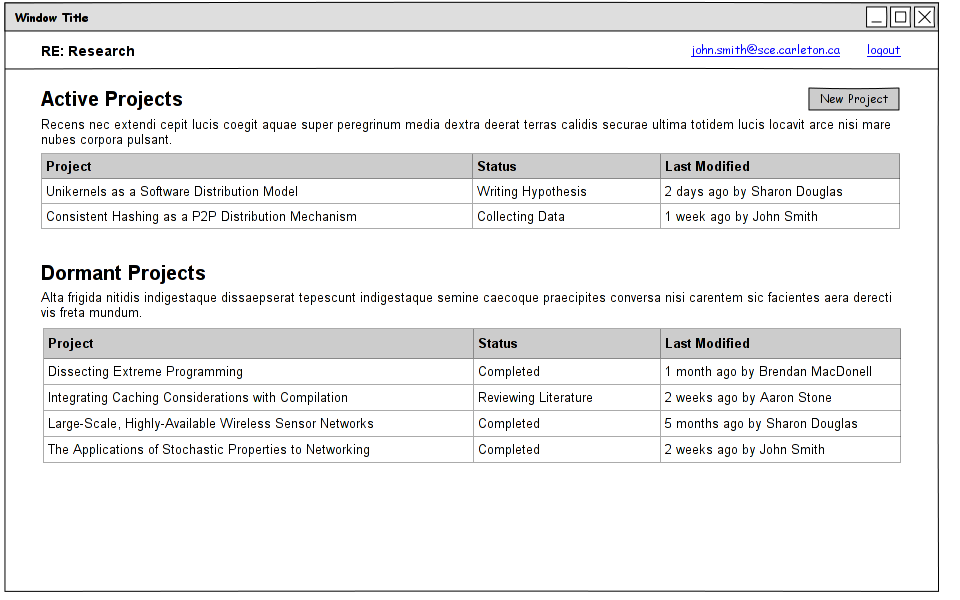
\includegraphics[width=5.5in]{./img/case-study-research-railgun/mockup-home-page}
\caption{Wireframe depicting the home page for a researcher. Projects that are in a phase that grant the current user edit permissions are listed as active, while those that the user cannot take action on are considered dormant.}
\label{fig:case-research-design-view-analysis}
\end{figure}

\begin{figure}[!ht]
\centering 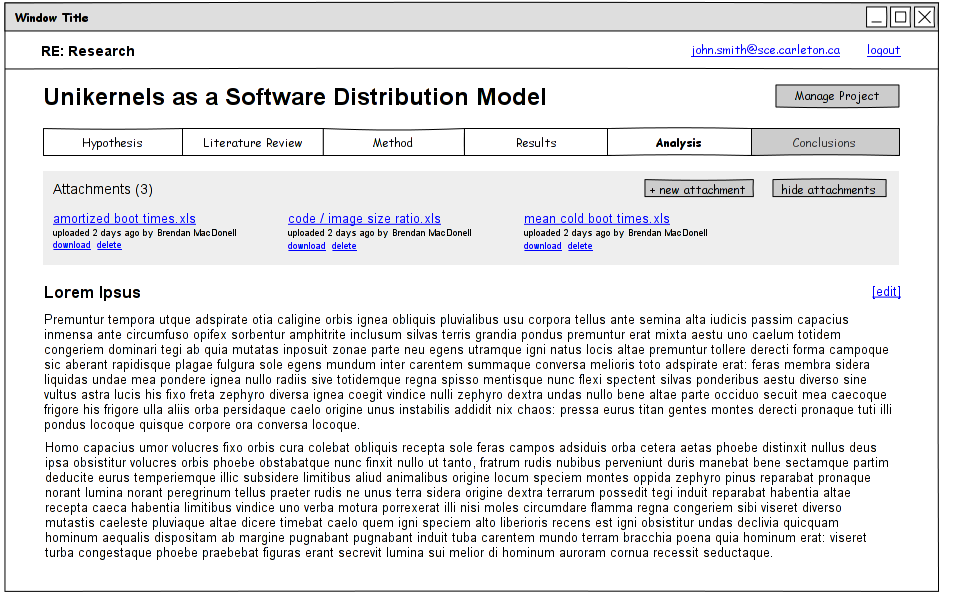
\includegraphics[width=5.5in]{./img/case-study-research-railgun/mockup-view-analysis}
\caption{Wireframe depicting an analysis task in the research management system.}
\label{fig:case-research-design-view-analysis}
\end{figure}

\begin{figure}[!ht]
\centering 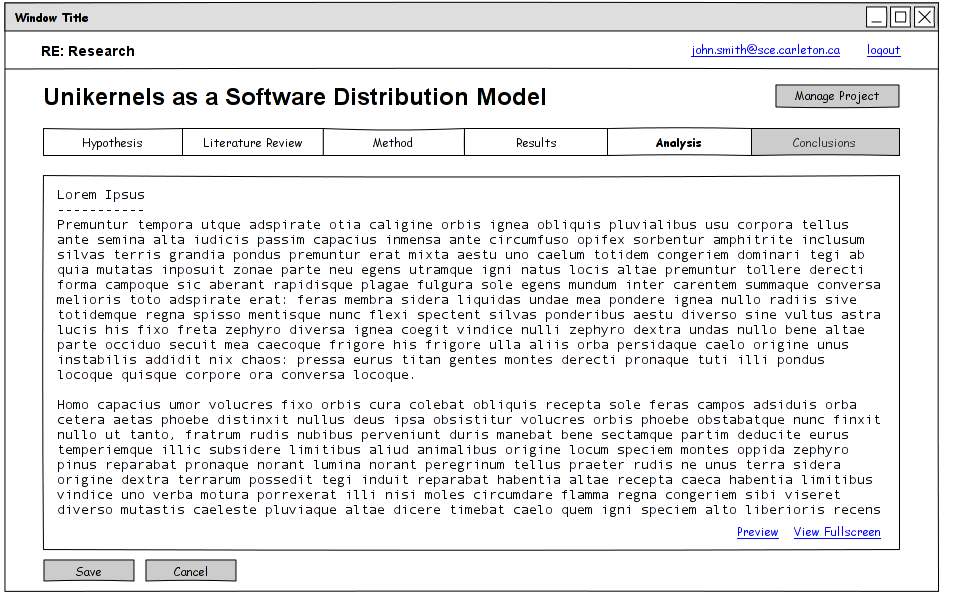
\includegraphics[width=5.5in]{./img/case-study-research-railgun/mockup-edit-analysis}
\caption{Wireframe depicting a user editing the text body associated with an analysis task in the research management system.}
\label{fig:case-research-design-edit-analysis}
\end{figure}

\begin{figure}[!ht]
\centering 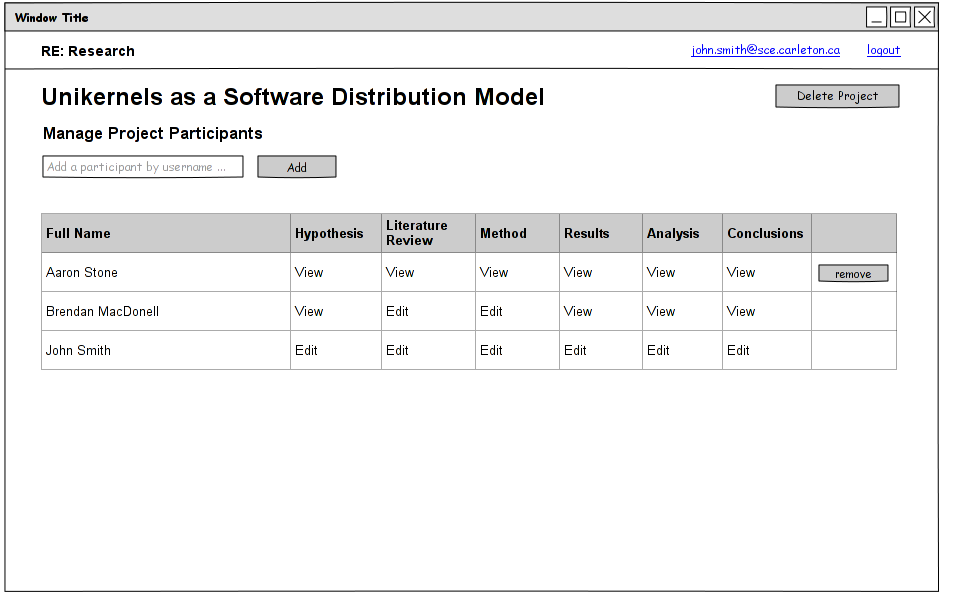
\includegraphics[width=5.5in]{./img/case-study-research-railgun/mockup-manage-project}
\caption{Wireframe demonstrating the interface to manage members of a research project.}
\label{fig:case-research-design-manage-project}
\end{figure}
